% Author working draft, revised from the supplied ICASSP project on 2026-09-22.
% This is not a submission-ready manuscript. See notes/AUTHOR_HANDOFF_ZH.md.
\documentclass[10pt,letterpaper]{article}
\usepackage{template/official/spconf}
\usepackage[T1]{fontenc}
\usepackage{amsmath,amssymb,graphicx,booktabs,array,tabularx}
\usepackage{balance}
\usepackage[hidelinks]{hyperref}
\hypersetup{
 pdftitle={PairSelect: Training-Free Token Selection for Efficient Weakly Supervised Video Anomaly Detection},
 pdfauthor={Zitong Qi; Yu Ji; Yihan Zhang; Ruihan Liu; Zhixiang Liu; Yu Pan; Jianbo Yu},
 pdfsubject={Author working draft; four-system, three-budget quality and scope-separated efficiency evaluation},
 pdfkeywords={WSVAD, PairSelect, training-free, token selection, ICASSP 2027}}
\setlength{\emergencystretch}{2em}
% Moderate positive float-to-text spacing; preserve template margins and body leading.
\setlength{\dbltextfloatsep}{12pt plus 2pt minus 2pt}
\setlength{\textfloatsep}{12pt plus 2pt minus 2pt}
\newcommand{\method}{PairSelect}
\newcommand{\tableinput}[1]{\csname @@input\endcsname{#1}}
\newcommand{\draftnote}[1]{\par\noindent\textit{Author working draft: #1}\par}
\newcommand{\norm}[1]{\left\lVert#1\right\rVert_2}
% Author block updated 2026-09-22 from the ICASSP 2027 submission form.
% ICASSP 2027 is NOT double blind. Do not anonymize the author block.
% Order below must match the submission system and the final PDF exactly.
%
% NOTE ON SYNTAX: spconf defines \name as
%     \def\name#1{\gdef\@name{{\em #1}\\}}
% so the argument is wrapped in an {\em ...} group. A "\\" inside that group
% cannot break the row of the title-block tabular and produces
% "! Missing } inserted". We therefore define \@name directly and place every
% "\\" outside the {\em ...} groups.
\makeatletter
\def\@name{{\em Zitong Qi$^{\star,1}$ \qquad Yu Ji$^{\dagger,1}$ \qquad Yihan Zhang$^{\star}$ \qquad Ruihan Liu$^{\dagger}$}\\[2pt]
{\em Zhixiang Liu$^{\dagger}$ \qquad Yu Pan$^{\star}$ \qquad Jianbo Yu$^{\dagger,\ddagger}$}}
\makeatother
\address{$^{\star}$Ningbo University, Ningbo, China \\
$^{\dagger}$Fudan University, Shanghai, China \\
$^{\ddagger}$Corresponding author \\
$^{1}$Zitong Qi and Yu Ji contributed equally to this work.}
% AUTHOR ACTION: e-mail addresses and the ORCiD IDs required by ICASSP 2027 are
% collected in the submission system only; they are deliberately not printed in
% this draft and must not be invented here. Confirm spelling, order and
% affiliations against the submission form before upload.

\title{PAIRSELECT: TRAINING-FREE TOKEN SELECTION FOR EFFICIENT\\WEAKLY SUPERVISED VIDEO ANOMALY DETECTION}
\begin{document}
% Venue-provided nine-point option; no margin or template modification.
\ninept
\maketitle
\begin{abstract}
Detecting rare events requires sustained observation, but not full computation for every internal token. We introduce PairSelect, a training-free operator that retains local, magnitude-guided representatives after six dense transformer blocks, without mixing their vectors or reducing input coverage. To assess generalization, we evaluate four weakly supervised video anomaly detection systems: VideoMAEv2-B, VideoMAE-B, and TimeSformer-B paired with a common UR-DMU detection-head architecture, and CLIP ViT-B/16 paired with DSANet, a recent state-of-the-art detector. Each UR-DMU head is trained separately on its encoder’s full dense-feature training set, and all four systems reuse their detector weights across token budgets. Across UCF-Crime and XD-Violence, 40\% nominal token deletion preserves near-dense performance in most configurations, with batch-32 encoder speedups of 1.22--1.28$\times$. With only mild performance degradation in most configurations, increasing deletion to 60\% delivers up to 1.47$\times$ encoder acceleration. These results demonstrate that PairSelect generalizes across visual representations and detection architectures, improving encoder efficiency without compression-specific retraining.
\end{abstract}
\begin{keywords}
video anomaly detection, weak supervision, token selection, training-free compression, efficient inference
\end{keywords}
\section{Introduction}
\label{sec:introduction}
% User-supplied conceptual artwork; original pixels retained for visual fidelity.
% Editable reconstruction and untouched reference page: pairselect_graphical_overview.drawio.
% Curve geometry is illustrative, not a new experimental result.
\begin{figure}[!t]
\centering
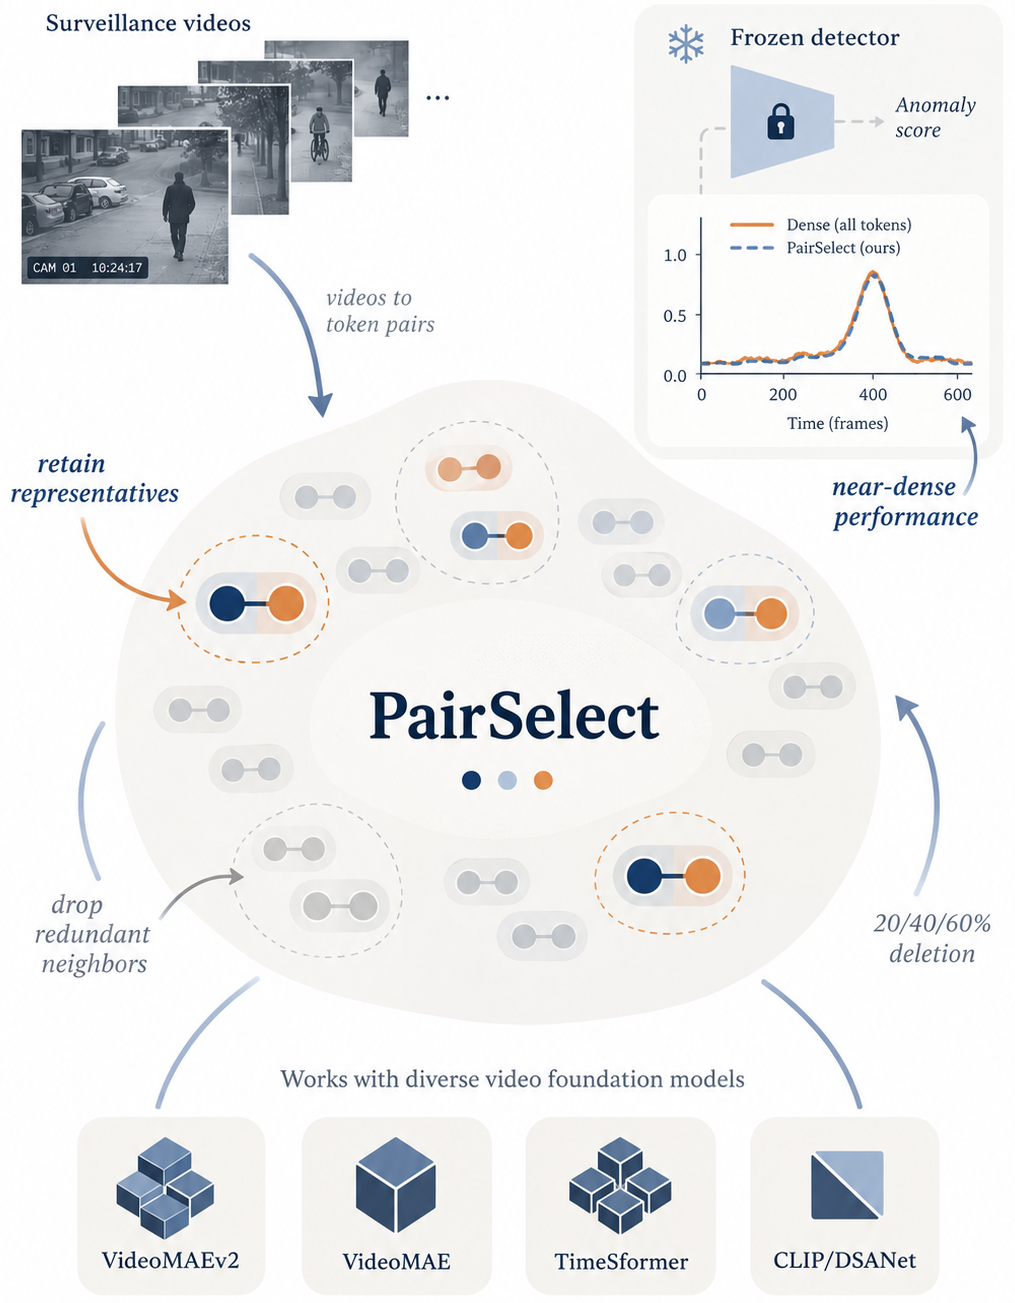
\includegraphics[width=\columnwidth]{figures/pairselect_graphical_overview.png}
\caption{Conceptual overview of \method{}: local representative selection at three deletion budgets with frozen detection across four systems. Score curves are schematic, not measured results.}
\label{fig:concept}
\end{figure}

% Full-width framework figure, updated from the user-approved draw.io.
% PNG is a 2x native render (3072 x 1728), cropped at canvas y=864
% to omit its baked-in caption. The LaTeX caption below is unchanged.
\begin{figure*}[!t]
\centering
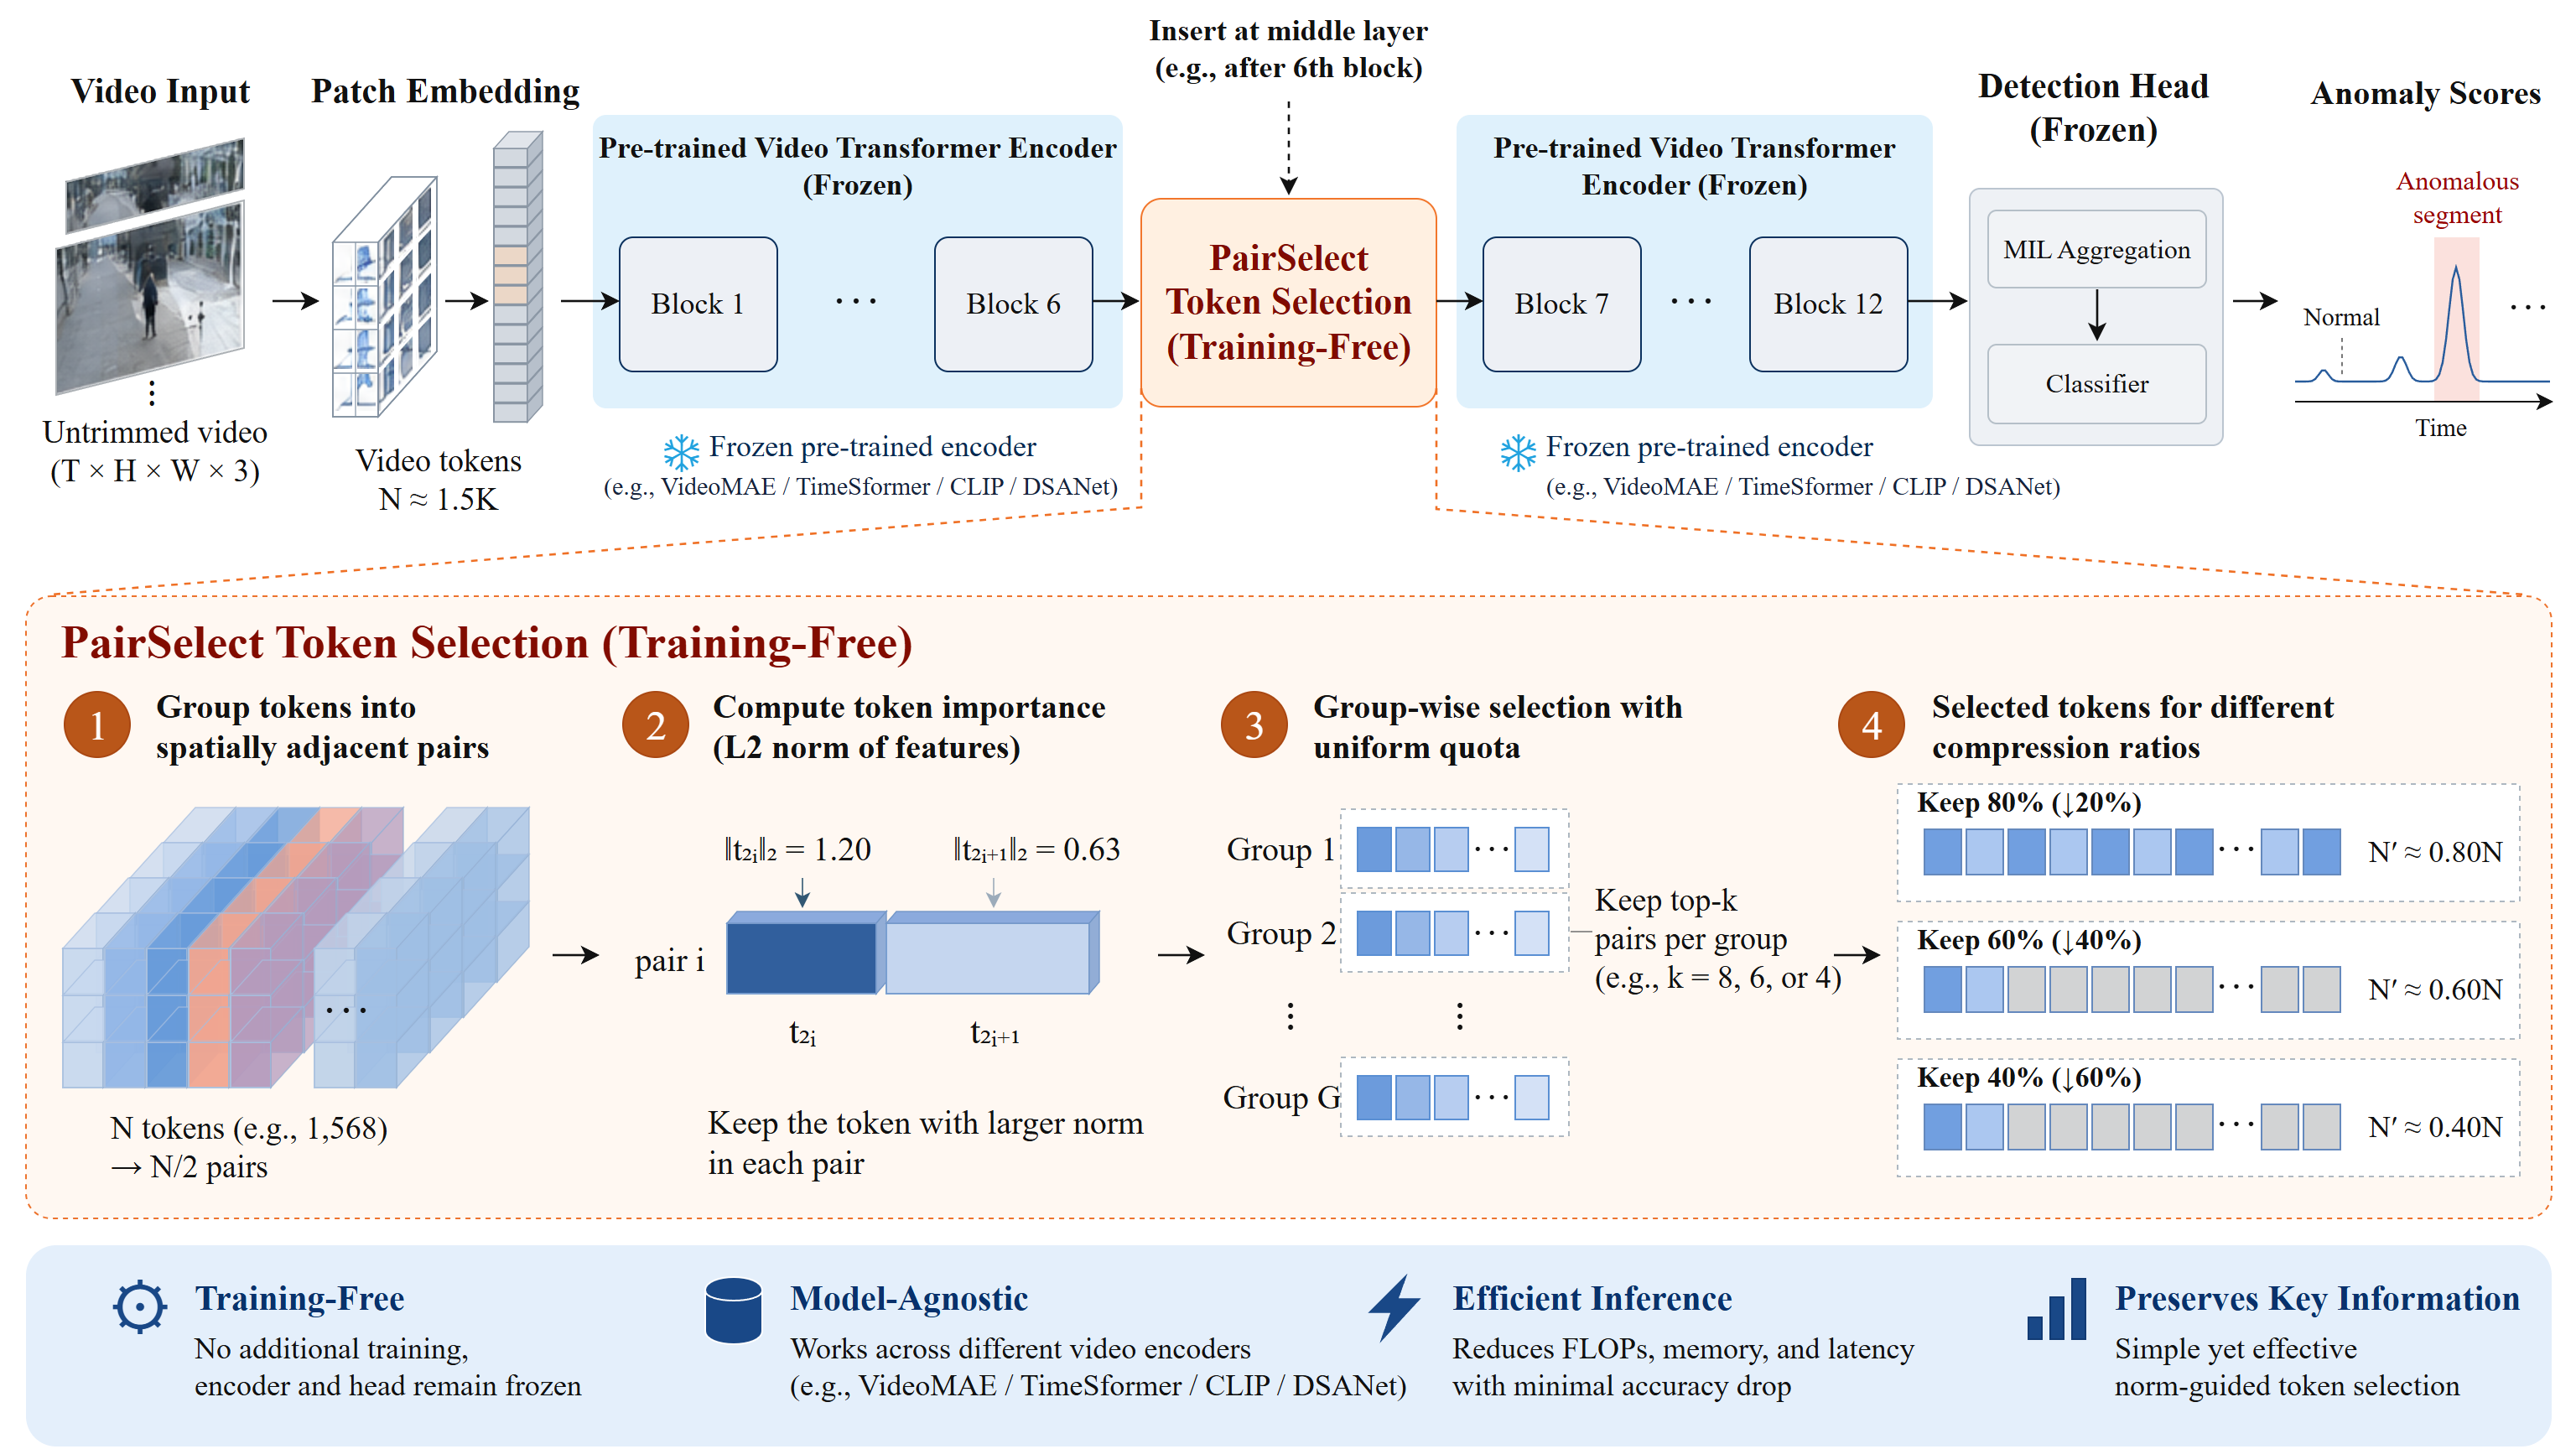
\includegraphics[width=\textwidth]{figures/pairselect_framework.png}
\caption{Overview of \method{}. Six dense blocks contextualize all tokens before local, magnitude-guided selection reduces the input to blocks 7--12. Group quotas control pair-member selection; divided attention retains complete spatial trajectories. The four systems reuse their original temporal sampling and detector weights; CLIP applies pair selection per image and preserves CLS.}
\label{fig:overview}
\end{figure*}

Video anomaly detection faces an asymmetric computational problem: unusual events are scarce, yet the system must process long stretches of ordinary activity to find them. Weakly supervised video anomaly detection (WSVAD) learns from video-level labels without knowing which snippets contain anomalies~\cite{sultani2018real,tian2021rtfm}. Contemporary systems combine pretrained visual representations with temporal detectors, from dual-memory models~\cite{zhou2023urdmu} to CLIP-based semantic alignment~\cite{wu2024vadclip,yin2026learning}. Their representations differ, but they share a deployment question: can an existing detector use less encoding computation without another training cycle?

Reducing the number of sampled clips also changes the temporal observations available to the detector. We instead preserve the original sampling schedule and reduce computation inside the visual encoder. \emph{The rarity of anomalous events does not imply that every internal token carries unique information.} Video redundancy supports masked pretraining~\cite{tong2022videomae,wang2023videomaev2}, while token sampling and merging demonstrate opportunities to process fewer representations~\cite{fayyaz2022ats,bolya2023tome}. This suggests allowing every token to participate in early contextualization, then continuing with locally selected representatives.

We propose \method{}, a non-mixing token selection operator for frozen WSVAD systems (Figs.~\ref{fig:concept} and~\ref{fig:overview}). Local pairing defines where candidates compete, group quotas distribute the budget, and activation magnitude determines member priority. Selected vectors are gathered without averaging. The same principle applies to video-patch representations and CLIP image patches; divided space--time attention instead selects complete spatial trajectories. Neither the visual encoder nor the detector is retrained after insertion or when the budget changes.

Our evaluation jointly covers four systems: VideoMAEv2-B, VideoMAE-B, and TimeSformer-B with their respective UR-DMU heads, and CLIP ViT-B/16 with the published DSANet weights. DSANet is a recent high-performance, state-of-the-art-level WSVAD system~\cite{yin2026learning}, making this a test of transfer across both visual representations and detector designs. We contribute the local selection rule, its architecture-aware application, and a complete three-budget quality--efficiency study on two datasets. At 40\% nominal deletion, most configurations retain near-dense quality; 60\% deletion offers greater encoder throughput with generally mild quality costs.

\section{Related Work}
\label{sec:related}
\textbf{Weakly supervised anomaly detection.}
Multiple-instance ranking~\cite{sultani2018real}, temporal feature magnitudes~\cite{tian2021rtfm}, and uncertainty-regulated memory~\cite{zhou2023urdmu} address weak supervision. VadCLIP adapts vision--language representations~\cite{wu2024vadclip}; DSANet disentangles normality and abnormality through semantic alignment~\cite{yin2026learning}. Our four-system study uses both UR-DMU and DSANet without changing their detector weights for compression. It is visual-only on both UCF-Crime and the audiovisual XD-Violence benchmark~\cite{wu2020xd}.

\textbf{Efficient visual representations.}
VideoMAE-family encoders use masked video pretraining~\cite{tong2022videomae,wang2023videomaev2}, whereas TimeSformer separates spatial and temporal attention~\cite{bertasius2021timesformer}. DynamicViT learns token predictors~\cite{rao2021dynamicvit}, EViT reorganizes token representations~\cite{liang2022evit}, and EVAD introduces task-aware token dropout for action detection~\cite{chen2023evad}. ATS and ToMe support reduction without additional training~\cite{fayyaz2022ats,bolya2023tome}. PairSelect focuses on locally constrained, non-mixing selection that can be inserted into an existing anomaly detector. In contrast, ESOM and LAVIDA reduce tokens within multimodal language-model pipelines~\cite{liu2026esom,dai2026lavida}. Our target is the visual-encoder cost of frozen temporal detection systems.

\section{PairSelect}
\label{sec:method}
\begin{table}[!b]
\centering\small
\caption{Actual token counts entering blocks 7--12. Headers specify nominal deletion; CLS is included when present. Video encoders count tokens per clip; CLIP counts per image.}
\label{tab:budgets}
\setlength{\tabcolsep}{3pt}
\begin{tabular}{@{}lrrrr@{}}
\toprule
Visual encoder + detector & Dense & 20\% & 40\% & 60\%\\
\midrule
\tableinput{tables/theory_rows}
\bottomrule
\end{tabular}
\end{table}
\begin{table*}[!t]
\centering\small
\caption{Four-system quality at every budget (0--100). Each cell reports the indicated two frame-level metrics; bold identifies the primary metric, not a ranking. On XD, the video systems use trapezoidal PR-AUC and DSANet uses step AP. CI is the paired 95\% interval for the primary-metric change at 40\% deletion, in percentage points.}
\label{tab:quality}
\setlength{\tabcolsep}{4pt}
\begin{tabular}{@{}lrrrrc@{}}
\toprule
System & Dense & Delete 20\% & Delete 40\% & Delete 60\% & CI of $\Delta_{40}$\\
\midrule
\tableinput{tables/quality_rows}
\bottomrule
\end{tabular}
\end{table*}


\subsection{Direct insertion into frozen systems}
Let $E_{1:b}$ and $E_{b+1:L}$ be the prefix and suffix of a pretrained visual encoder, $R$ its readout, and $H$ its temporal detection head. For scheduled visual inputs $\{v_t\}_{t=1}^{M}$,
\begin{equation}
 z_t^{(r)}=R\!\left(E_{b+1:L}\!\left(S_r(E_{1:b}(v_t))\right)\right),
 \quad \hat{\boldsymbol y}^{(r)}=H(\{z_t^{(r)}\}_{t=1}^{M}).
 \label{eq:pipeline}
\end{equation}
Only the selection operator $S_r$ is inserted, with retention ratio $r$. All four visual encoders use $L=12$, $b=6$. The original input schedule, feature dimension, temporal aggregation, and head weights are preserved. For the three video backbones, each UR-DMU head is trained once on the corresponding dense training features; DSANet uses the authors' released detector weights. \emph{Training-free} refers to inserting and changing the compression operator, not to training the original systems.

Local redundancy motivates comparisons among neighboring patches, while selection avoids introducing additional vector mixtures at the insertion point. Activation magnitude provides an inexpensive preference, inspired by magnitude-aware sampling~\cite{fayyaz2022ats}. It is not an anomaly probability~\cite{darcet2024registers}; the local quota prevents an unconstrained global ranking from concentrating the entire budget in a few regions.

\subsection{Local quotas and member priority}
For VideoMAE, VideoMAEv2, and CLIP, spatially adjacent horizontal patches form pairs ordered by native coordinates. Each consecutive group contains at most ten patch tokens (five pairs). A group of $n_g$ tokens receives
\begin{equation}
 q_g(r)=\lfloor rn_g+\tfrac12\rfloor,
 \qquad r\in\{0.8,0.6,0.4\}.
 \label{eq:quota}
\end{equation}
For pair $j$ with members $(x_{j,0},x_{j,1})$, define
\begin{equation}
 a_j=\arg\max_{u\in\{0,1\}}\norm{x_{j,u}},\quad
 s_j=\max_{u\in\{0,1\}}\norm{x_{j,u}}.
 \label{eq:score}
\end{equation}
Let $w_j=x_{j,a_j}$ and $\ell_j=x_{j,1-a_j}$. If $\pi$ sorts the group's $m_g$ pairs by descending $s_j$, the priority sequence is
\begin{equation}
 \mathcal P_g=(w_{\pi_1},\ldots,w_{\pi_{m_g}},
                 \ell_{\pi_1},\ldots,\ell_{\pi_{m_g}}).
 \label{eq:priority}
\end{equation}
The first $q_g$ entries are retained and restored to native index order before gathering. Ties preserve native order. At 20\% and 40\% deletion, every pair in a full group retains a representative, with three or one additional members; 60\% deletion retains four of five representatives. Selected vectors are neither averaged nor rescaled. CLIP applies the rule independently per image and always retains CLS, yielding the counts in Table~\ref{tab:budgets}.

\subsection{Structure-aware adaptation}
For TimeSformer, the selection unit is a complete spatial trajectory of $T$ tokens, scored by its maximum member norm. Each group of ten trajectories retains its top $q_g$. The current bridge rounds the total spatial count down to a multiple of native width $W$, removing excess quota from tail groups:
\begin{equation}
 P'=W\left\lfloor\frac{\sum_g q_g(r)}{W}\right\rfloor,
 \qquad K=TP'+1.
 \label{eq:trajectory}
\end{equation}
With $P=196$, $T=8$, and $W=14$, the three budgets retain 154, 112, and 70 trajectories plus CLS. Actual token deletion is 21.41\%, 42.83\%, and 64.24\%; this alignment constraint is implementation-specific. Video-encoder bridges use a fixed quota-slot skeleton with approximate spatial anchors while retaining trajectory time indices. CLIP gathers the already position-embedded patch states in native order and preserves its CLS readout. These adaptations keep the detector interface unchanged.

\section{Experiments}
\label{sec:experiments}
\begin{table*}[t]
\centering\small
\caption{Efficiency of dense and PairSelect configurations. $F_{\rm blocks}$ is an analytical principal-block estimate (1 MAC = 2 FLOPs). Full-encoder FLOPs, latency, throughput, and peak allocated/reserved memory remain unmeasured.}
\label{tab:efficiency}
\setlength{\tabcolsep}{5.5pt}
\begin{tabular}{@{}llrrrrrr@{}}
\toprule
Encoder & Delete & Tokens & $F_{\rm blocks}$ & $F_{\rm full}$ & Latency & Throughput & Peak memory\\
 & & & GFLOPs & GFLOPs & ms/clip & clips/s & alloc./res. GiB\\
\midrule
\tableinput{tables/efficiency_rows}
\bottomrule
\end{tabular}
\end{table*}

\subsection{Four-system evaluation}
We evaluate on UCF-Crime~\cite{sultani2018real} (1,610 training and 290 test videos) and XD-Violence~\cite{wu2020xd} (3,950 accepted training and all 800 test videos; four declared training files fail source-integrity checks). VideoMAEv2-B, VideoMAE-B, and TimeSformer-B use pretrained encoders and separate UR-DMU heads trained on the corresponding complete accepted training sets. The heads use 200 temporal bins, 64 normal and 64 anomalous bags per step, Adam with learning rate $10^{-4}$ and weight decay $5\!\times\!10^{-5}$, and the final checkpoint after 3,000 steps. CLIP ViT-B/16 uses the authors' released UCF/XD DSANet checkpoints~\cite{yin2026learning}, with no DSANet training in this study. All four systems reuse their dense detector at every budget.

Each system preserves its native input schedule and temporal scoring protocol. VideoMAEv2-B and VideoMAE-B use 16-frame inputs, TimeSformer-B uses eight-frame inputs, and CLIP ViT-B/16 processes sampled frames under its fixed raw-video protocol, all at 224$\times$224 resolution. Detector weights and scoring rules remain fixed across token budgets, with the coarse branch used for DSANet. The CLIP dense reference is extracted from the same raw videos as its compressed counterparts, ensuring that the comparison uses the evaluated raw-video pipeline rather than a score obtained from externally released features.

UCF uses frame ROC-AUC as primary metric and also reports step AP. On XD, the three video systems use trapezoidal PR-AUC with the fixed 16-frame prefix alignment, while DSANet uses step AP. Table~\ref{tab:quality} separates both integration definitions. Paired video-level, weak-label-stratified bootstrap uses 10,000 resamples; all-budget intervals are retained with the result exports.

\subsection{Quality across systems and budgets}
At 40\% nominal deletion, \method{} is nearly lossless in most configurations. The three video systems change UCF AUC by $+0.39$, $-0.16$, and approximately $0.00$ points, and XD PR-AUC by $+0.32$, $+0.61$, and $+0.68$. DSANet changes UCF AUC by $-0.90$ and XD step AP by $-0.24$ points, retaining 87.97 AUC and 85.35 AP. UCF step AP is also stable: 19.29$\to$19.60, 18.82$\to$18.99, 20.37$\to$20.90, and 34.74$\to$34.36 across the four systems. No compression-specific training is used to obtain these results.

Increasing deletion to 60\% generally incurs mild degradation while preserving high detection quality. Several configurations improve, and the three largest primary-metric drops are DSANet/UCF ($-1.80$), DSANet/XD ($-1.22$), and VideoMAE/UCF ($-1.05$ points). This extends the usable reduction range across video-pretrained and image--text-pretrained representations and across UR-DMU and DSANet. The two XD metrics need not move together: VideoMAE at 60\% gains 0.78 PR-AUC points but loses 1.39 step-AP points; both are retained in the table. Near-lossless describes point estimates rather than a blanket statistical guarantee: among DSANet budgets, only XD at 20\% has its 95\% lower bound above the predeclared $-0.5$-point margin.

\subsection{Encoder efficiency}
Table~\ref{tab:efficiency} compares batch-32 encoder efficiency across budgets using XD training inputs. Encoder timing includes embedding, selection, gathering, all blocks, and readout. Video-encoder B32 tests use two fixed training videos, 20 warmups and 40 synchronized samples; CLIP uses three processes, 20 warmups and 40 timed samples per setting. Arithmetic values cover the principal twelve blocks (one MAC is two FLOPs), not a full-model profiler estimate.

We evaluate encoder efficiency using speedup relative to each system’s dense counterpart at the same batch size. At batch size 32, PairSelect achieves encoder speedups of 1.22--1.28$\times$ at 40\% nominal token deletion while preserving near-dense detection performance in most configurations. Increasing deletion to 60\% raises encoder speedups to 1.33--1.47$\times$, with generally mild performance degradation. These results highlight a favorable accuracy--efficiency trade-off: PairSelect reduces internal token computation while preserving input coverage and reusing the same detector weights across budgets.

\balance
\section{Scope and Discussion}
\label{sec:limitations}
Evaluation covers three backbones, two attention families, and one detector family; behavior may vary across architectures, datasets, and metrics. Insertion depth and group size are fixed, not optimized. Standard external reducers such as ATS or ToMe remain to be compared. Earlier diagnostics accessed UCF test data, so development was not wholly test-blind. All additional budgets must be reported, without post-hoc selection implying an independently validated optimum.

Local coverage neither identifies anomalies nor guarantees short-event preservation; anchor positions remain approximate. Reduction affects internal activations, not model weights, output dimension, or detector input count. Deployment benefits depend jointly on measured computation, execution overhead, and hardware behavior.
\section{Conclusion}
\label{sec:conclusion}
\method{} reduces internal video-token computation without reducing the existing clip schedule or retraining the anomaly detection pipeline. Local quotas, magnitude-guided representatives, and non-mixing gathers provide a configurable selection rule for joint and divided attention. The completed middle-budget results show small primary-metric point-estimate changes across three encoders and two datasets, alongside a 21.75--23.04\% analytical reduction in principal-block operations. Completing the budget ladder and hardware measurements will determine which operating points offer a useful quality--efficiency trade-off in practice.

\label{lasttechnical}
% The fifth page is not a technical appendix. Keep every technical float before this boundary.
\clearpage
\balance
\section{Compliance with Ethical Standards}
This research uses existing UCF-Crime and XD-Violence benchmarks and does not introduce participant recruitment or newly collected personal data. The experiments concern offline benchmark evaluation, not deployment decisions about individuals.
% Authors must confirm permissions, institutional ethics requirements, funding,
% conflicts, and the venue's AI-use requirements before any submission.
% See notes/REBUILD_HANDOFF.md; no approval or funding status is invented here.

\begingroup
\small
\bibliographystyle{template/official/IEEEbib}
\bibliography{references}
\endgroup
\end{document}
